\documentclass[twoside]{book}

% Packages required by doxygen
\usepackage{fixltx2e}
\usepackage{calc}
\usepackage{doxygen}
\usepackage[export]{adjustbox} % also loads graphicx
\usepackage{graphicx}
\usepackage[utf8]{inputenc}
\usepackage{makeidx}
\usepackage{multicol}
\usepackage{multirow}
\PassOptionsToPackage{warn}{textcomp}
\usepackage{textcomp}
\usepackage[nointegrals]{wasysym}
\usepackage[table]{xcolor}

% Font selection
\usepackage[T1]{fontenc}
\usepackage[scaled=.90]{helvet}
\usepackage{courier}
\usepackage{amssymb}
\usepackage{sectsty}
\renewcommand{\familydefault}{\sfdefault}
\allsectionsfont{%
  \fontseries{bc}\selectfont%
  \color{darkgray}%
}
\renewcommand{\DoxyLabelFont}{%
  \fontseries{bc}\selectfont%
  \color{darkgray}%
}
\newcommand{\+}{\discretionary{\mbox{\scriptsize$\hookleftarrow$}}{}{}}

% Page & text layout
\usepackage{geometry}
\geometry{%
  a4paper,%
  top=2.5cm,%
  bottom=2.5cm,%
  left=2.5cm,%
  right=2.5cm%
}
\tolerance=750
\hfuzz=15pt
\hbadness=750
\setlength{\emergencystretch}{15pt}
\setlength{\parindent}{0cm}
\setlength{\parskip}{3ex plus 2ex minus 2ex}
\makeatletter
\renewcommand{\paragraph}{%
  \@startsection{paragraph}{4}{0ex}{-1.0ex}{1.0ex}{%
    \normalfont\normalsize\bfseries\SS@parafont%
  }%
}
\renewcommand{\subparagraph}{%
  \@startsection{subparagraph}{5}{0ex}{-1.0ex}{1.0ex}{%
    \normalfont\normalsize\bfseries\SS@subparafont%
  }%
}
\makeatother

% Headers & footers
\usepackage{fancyhdr}
\pagestyle{fancyplain}
\fancyhead[LE]{\fancyplain{}{\bfseries\thepage}}
\fancyhead[CE]{\fancyplain{}{}}
\fancyhead[RE]{\fancyplain{}{\bfseries\leftmark}}
\fancyhead[LO]{\fancyplain{}{\bfseries\rightmark}}
\fancyhead[CO]{\fancyplain{}{}}
\fancyhead[RO]{\fancyplain{}{\bfseries\thepage}}
\fancyfoot[LE]{\fancyplain{}{}}
\fancyfoot[CE]{\fancyplain{}{}}
\fancyfoot[RE]{\fancyplain{}{\bfseries\scriptsize Generated by Doxygen }}
\fancyfoot[LO]{\fancyplain{}{\bfseries\scriptsize Generated by Doxygen }}
\fancyfoot[CO]{\fancyplain{}{}}
\fancyfoot[RO]{\fancyplain{}{}}
\renewcommand{\footrulewidth}{0.4pt}
\renewcommand{\chaptermark}[1]{%
  \markboth{#1}{}%
}
\renewcommand{\sectionmark}[1]{%
  \markright{\thesection\ #1}%
}

% Indices & bibliography
\usepackage{natbib}
\usepackage[titles]{tocloft}
\setcounter{tocdepth}{3}
\setcounter{secnumdepth}{5}
\makeindex

% Hyperlinks (required, but should be loaded last)
\usepackage{ifpdf}
\ifpdf
  \usepackage[pdftex,pagebackref=true]{hyperref}
\else
  \usepackage[ps2pdf,pagebackref=true]{hyperref}
\fi
\hypersetup{%
  colorlinks=true,%
  linkcolor=blue,%
  citecolor=blue,%
  unicode%
}

% Custom commands
\newcommand{\clearemptydoublepage}{%
  \newpage{\pagestyle{empty}\cleardoublepage}%
}

\usepackage{caption}
\captionsetup{labelsep=space,justification=centering,font={bf},singlelinecheck=off,skip=4pt,position=top}

%===== C O N T E N T S =====

\begin{document}

% Titlepage & ToC
\hypersetup{pageanchor=false,
             bookmarksnumbered=true,
             pdfencoding=unicode
            }
\pagenumbering{roman}
\begin{titlepage}
\vspace*{7cm}
\begin{center}%
{\Large My Project }\\
\vspace*{1cm}
{\large Generated by Doxygen 1.8.11}\\
\end{center}
\end{titlepage}
\clearemptydoublepage
\tableofcontents
\clearemptydoublepage
\pagenumbering{arabic}
\hypersetup{pageanchor=true}

%--- Begin generated contents ---
\chapter{File Index}
\section{File List}
Here is a list of all files with brief descriptions\+:\begin{DoxyCompactList}
\item\contentsline{section}{\hyperlink{assimp_8c}{assimp.\+c} \\*Utilisation de G\+L4\+Dummies et Lib Assimp pour chargement de sc�nes }{\pageref{assimp_8c}}{}
\item\contentsline{section}{\hyperlink{assimp_8h}{assimp.\+h} \\*Fonctionalit�s pour utilisation de lib Assimp sous G\+L4\+Dummies }{\pageref{assimp_8h}}{}
\item\contentsline{section}{\hyperlink{window_8cpp}{window.\+cpp} }{\pageref{window_8cpp}}{}
\end{DoxyCompactList}

\chapter{File Documentation}
\hypertarget{assimp_8c}{}\section{assimp.\+c File Reference}
\label{assimp_8c}\index{assimp.\+c@{assimp.\+c}}


utilisation de G\+L4\+Dummies et Lib Assimp pour chargement de sc�nes.  


{\ttfamily \#include $<$G\+L4\+D/gl4duw\+\_\+\+S\+D\+L2.\+h$>$}\\*
{\ttfamily \#include $<$S\+D\+L\+\_\+image.\+h$>$}\\*
{\ttfamily \#include $<$assimp/cimport.\+h$>$}\\*
{\ttfamily \#include $<$assimp/scene.\+h$>$}\\*
{\ttfamily \#include $<$assimp/postprocess.\+h$>$}\\*
{\ttfamily \#include $<$assert.\+h$>$}\\*
Include dependency graph for assimp.\+c\+:
\nopagebreak
\begin{figure}[H]
\begin{center}
\leavevmode
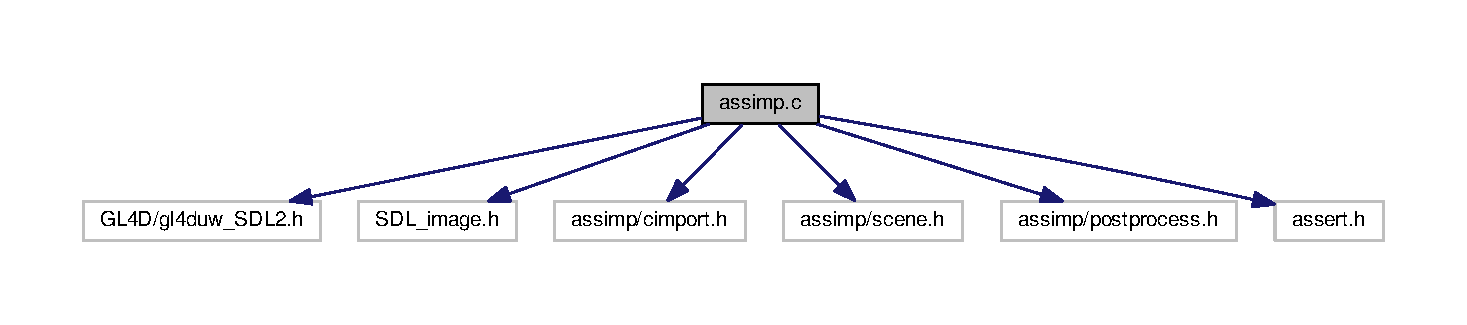
\includegraphics[width=350pt]{assimp_8c__incl}
\end{center}
\end{figure}
\subsection*{Macros}
\begin{DoxyCompactItemize}
\item 
\#define \hyperlink{assimp_8c_aa1e54f63f92837dac507492611a6986d}{\+\_\+nb\+\_\+max\+\_\+item}~30
\item 
\#define \hyperlink{assimp_8c_ae19f66e94255e323687e3dcdd5362125}{aisgl\+\_\+min}(x,  y)~(x$<$y?x\+:y)
\item 
\#define \hyperlink{assimp_8c_a5d7d752ed7ce95f82f595ac2e5e300aa}{aisgl\+\_\+max}(x,  y)~(y$>$x?y\+:x)
\end{DoxyCompactItemize}
\subsection*{Functions}
\begin{DoxyCompactItemize}
\item 
static void \hyperlink{assimp_8c_a2eece74effe5ff11aa569a84e63843ab}{get\+\_\+bounding\+\_\+box\+\_\+for\+\_\+node} (const struct ai\+Node $\ast$nd, struct ai\+Vector3D $\ast$min, struct ai\+Vector3D $\ast$max, struct ai\+Matrix4x4 $\ast$trafo, G\+Luint id)
\item 
static void \hyperlink{assimp_8c_a0f8cdb4671df4425602a2392ddbfdc39}{get\+\_\+bounding\+\_\+box} (struct ai\+Vector3D $\ast$min, struct ai\+Vector3D $\ast$max, G\+Luint id)
\item 
static void \hyperlink{assimp_8c_af9bda34ebe99a84f2e23617512cdbc91}{color4\+\_\+to\+\_\+float4} (const struct ai\+Color4D $\ast$c, float f\mbox{[}4\mbox{]})
\item 
static void \hyperlink{assimp_8c_ac786c5ece13cc71bc1124ba2bfecd31f}{set\+\_\+float4} (float f\mbox{[}4\mbox{]}, float a, float b, float c, float d)
\item 
static void \hyperlink{assimp_8c_a8e9bd18ccc4c4ef522837d732764f35b}{apply\+\_\+material} (const struct ai\+Material $\ast$mtl)
\item 
static void \hyperlink{assimp_8c_a270f111cfc21a76d5fbdba7f5dcf0b04}{scene\+Mk\+V\+A\+Os} (const struct ai\+Scene $\ast$sc, const struct ai\+Node $\ast$nd, G\+Luint $\ast$ivao, G\+Luint id)
\item 
static void \hyperlink{assimp_8c_a5d18bad9b596e4d08568189cf15cdab2}{scene\+Draw\+V\+A\+Os} (const struct ai\+Scene $\ast$sc, const struct ai\+Node $\ast$nd, G\+Luint $\ast$ivao, G\+Luint id)
\item 
static int \hyperlink{assimp_8c_a28355c3df9599a33526a2357fc27d611}{scene\+Nb\+Meshes} (const struct ai\+Scene $\ast$sc, const struct ai\+Node $\ast$nd, int subtotal)
\item 
static int \hyperlink{assimp_8c_a790a34d309ef3cdea306b092464be9a5}{loadasset} (const char $\ast$path, G\+Luint id)
\item 
void \hyperlink{assimp_8c_a05bb0781cb0c80b6585189c94850654a}{assimp\+Init} (const char $\ast$filename, G\+Luint id)
\begin{DoxyCompactList}\small\item\em modification du Assimp.\+c avec l\textquotesingle{}ajout d\textquotesingle{}un id afin de charger plusieurs objets diff�rents en m�me temps \end{DoxyCompactList}\item 
void \hyperlink{assimp_8c_a18a5a0391db704631c22f172fdd23981}{assimp\+Draw\+Scene} (G\+Luint id)
\item 
void \hyperlink{assimp_8c_a0c1f6c204843bd061140485cb4387622}{assimp\+Quit} (void)
\end{DoxyCompactItemize}
\subsection*{Variables}
\begin{DoxyCompactItemize}
\item 
static const struct ai\+Scene $\ast$ \hyperlink{assimp_8c_a78a06589c0da50b28334f43462b9f5f4}{\+\_\+scene} \mbox{[}\hyperlink{assimp_8c_aa1e54f63f92837dac507492611a6986d}{\+\_\+nb\+\_\+max\+\_\+item}\mbox{]}
\item 
static struct ai\+Vector3D \hyperlink{assimp_8c_a376ff4bcd2164265d4195259177d1f2e}{\+\_\+scene\+\_\+min} \mbox{[}\hyperlink{assimp_8c_aa1e54f63f92837dac507492611a6986d}{\+\_\+nb\+\_\+max\+\_\+item}\mbox{]}
\item 
static struct ai\+Vector3D \hyperlink{assimp_8c_a5ba9f7e2395e09f002de216c46d502d2}{\+\_\+scene\+\_\+max} \mbox{[}\hyperlink{assimp_8c_aa1e54f63f92837dac507492611a6986d}{\+\_\+nb\+\_\+max\+\_\+item}\mbox{]}
\item 
static struct ai\+Vector3D \hyperlink{assimp_8c_aed18c244c1ebab879376aabe0f3d9a3e}{\+\_\+scene\+\_\+center} \mbox{[}\hyperlink{assimp_8c_aa1e54f63f92837dac507492611a6986d}{\+\_\+nb\+\_\+max\+\_\+item}\mbox{]}
\item 
static G\+Luint $\ast$ \hyperlink{assimp_8c_acf7c96d567c0fcef9ea77572dcfd88af}{\+\_\+vaos} \mbox{[}\hyperlink{assimp_8c_aa1e54f63f92837dac507492611a6986d}{\+\_\+nb\+\_\+max\+\_\+item}\mbox{]}
\item 
static G\+Luint $\ast$ \hyperlink{assimp_8c_a35fdd8b2c1e2cf34f7df96e5f92e86a2}{\+\_\+buffers} \mbox{[}\hyperlink{assimp_8c_aa1e54f63f92837dac507492611a6986d}{\+\_\+nb\+\_\+max\+\_\+item}\mbox{]}
\item 
static G\+Luint $\ast$ \hyperlink{assimp_8c_a4a8a40d79df302927635f3674ad73394}{\+\_\+counts} \mbox{[}\hyperlink{assimp_8c_aa1e54f63f92837dac507492611a6986d}{\+\_\+nb\+\_\+max\+\_\+item}\mbox{]}
\item 
static G\+Luint $\ast$ \hyperlink{assimp_8c_ad1975cc80f02b47a040d4d6a60da6a67}{\+\_\+textures} \mbox{[}\hyperlink{assimp_8c_aa1e54f63f92837dac507492611a6986d}{\+\_\+nb\+\_\+max\+\_\+item}\mbox{]}
\item 
static G\+Luint \hyperlink{assimp_8c_a74ba65601d2391c2118eb47882b3b974}{\+\_\+nb\+Meshes} \mbox{[}\hyperlink{assimp_8c_aa1e54f63f92837dac507492611a6986d}{\+\_\+nb\+\_\+max\+\_\+item}\mbox{]}
\item 
static G\+Luint \hyperlink{assimp_8c_ac21bd89c19f2293fe4f3b87a09fe285d}{\+\_\+nb\+Textures} \mbox{[}\hyperlink{assimp_8c_aa1e54f63f92837dac507492611a6986d}{\+\_\+nb\+\_\+max\+\_\+item}\mbox{]}
\end{DoxyCompactItemize}


\subsection{Detailed Description}
utilisation de G\+L4\+Dummies et Lib Assimp pour chargement de sc�nes. 

Modification de l\textquotesingle{}exemple fourni par lib Assimp utilisant GL $<$ 3 et G\+L\+UT et upgrade avec utilisation des V\+A\+O/\+V\+BO et matrices et shaders G\+L4dummies.

\begin{DoxyAuthor}{Author}
Vincent Boyer et Far�s Belhadj \{boyer, amsi\}.univ-\/paris8.\+fr 
\end{DoxyAuthor}
\begin{DoxyDate}{Date}
February 14 2017 
\end{DoxyDate}


\subsection{Macro Definition Documentation}
\index{assimp.\+c@{assimp.\+c}!\+\_\+nb\+\_\+max\+\_\+item@{\+\_\+nb\+\_\+max\+\_\+item}}
\index{\+\_\+nb\+\_\+max\+\_\+item@{\+\_\+nb\+\_\+max\+\_\+item}!assimp.\+c@{assimp.\+c}}
\subsubsection[{\texorpdfstring{\+\_\+nb\+\_\+max\+\_\+item}{_nb_max_item}}]{\setlength{\rightskip}{0pt plus 5cm}\#define \+\_\+nb\+\_\+max\+\_\+item~30}\hypertarget{assimp_8c_aa1e54f63f92837dac507492611a6986d}{}\label{assimp_8c_aa1e54f63f92837dac507492611a6986d}
\index{assimp.\+c@{assimp.\+c}!aisgl\+\_\+max@{aisgl\+\_\+max}}
\index{aisgl\+\_\+max@{aisgl\+\_\+max}!assimp.\+c@{assimp.\+c}}
\subsubsection[{\texorpdfstring{aisgl\+\_\+max}{aisgl_max}}]{\setlength{\rightskip}{0pt plus 5cm}\#define aisgl\+\_\+max(
\begin{DoxyParamCaption}
\item[{}]{x, }
\item[{}]{y}
\end{DoxyParamCaption}
)~(y$>$x?y\+:x)}\hypertarget{assimp_8c_a5d7d752ed7ce95f82f595ac2e5e300aa}{}\label{assimp_8c_a5d7d752ed7ce95f82f595ac2e5e300aa}
\index{assimp.\+c@{assimp.\+c}!aisgl\+\_\+min@{aisgl\+\_\+min}}
\index{aisgl\+\_\+min@{aisgl\+\_\+min}!assimp.\+c@{assimp.\+c}}
\subsubsection[{\texorpdfstring{aisgl\+\_\+min}{aisgl_min}}]{\setlength{\rightskip}{0pt plus 5cm}\#define aisgl\+\_\+min(
\begin{DoxyParamCaption}
\item[{}]{x, }
\item[{}]{y}
\end{DoxyParamCaption}
)~(x$<$y?x\+:y)}\hypertarget{assimp_8c_ae19f66e94255e323687e3dcdd5362125}{}\label{assimp_8c_ae19f66e94255e323687e3dcdd5362125}


\subsection{Function Documentation}
\index{assimp.\+c@{assimp.\+c}!apply\+\_\+material@{apply\+\_\+material}}
\index{apply\+\_\+material@{apply\+\_\+material}!assimp.\+c@{assimp.\+c}}
\subsubsection[{\texorpdfstring{apply\+\_\+material(const struct ai\+Material $\ast$mtl)}{apply_material(const struct aiMaterial *mtl)}}]{\setlength{\rightskip}{0pt plus 5cm}static void apply\+\_\+material (
\begin{DoxyParamCaption}
\item[{const struct ai\+Material $\ast$}]{mtl}
\end{DoxyParamCaption}
)\hspace{0.3cm}{\ttfamily [static]}}\hypertarget{assimp_8c_a8e9bd18ccc4c4ef522837d732764f35b}{}\label{assimp_8c_a8e9bd18ccc4c4ef522837d732764f35b}
\index{assimp.\+c@{assimp.\+c}!assimp\+Draw\+Scene@{assimp\+Draw\+Scene}}
\index{assimp\+Draw\+Scene@{assimp\+Draw\+Scene}!assimp.\+c@{assimp.\+c}}
\subsubsection[{\texorpdfstring{assimp\+Draw\+Scene(\+G\+Luint id)}{assimpDrawScene(GLuint id)}}]{\setlength{\rightskip}{0pt plus 5cm}void assimp\+Draw\+Scene (
\begin{DoxyParamCaption}
\item[{G\+Luint}]{id}
\end{DoxyParamCaption}
)}\hypertarget{assimp_8c_a18a5a0391db704631c22f172fdd23981}{}\label{assimp_8c_a18a5a0391db704631c22f172fdd23981}
\index{assimp.\+c@{assimp.\+c}!assimp\+Init@{assimp\+Init}}
\index{assimp\+Init@{assimp\+Init}!assimp.\+c@{assimp.\+c}}
\subsubsection[{\texorpdfstring{assimp\+Init(const char $\ast$filename, G\+Luint id)}{assimpInit(const char *filename, GLuint id)}}]{\setlength{\rightskip}{0pt plus 5cm}void assimp\+Init (
\begin{DoxyParamCaption}
\item[{const char $\ast$}]{filename, }
\item[{G\+Luint}]{id}
\end{DoxyParamCaption}
)}\hypertarget{assimp_8c_a05bb0781cb0c80b6585189c94850654a}{}\label{assimp_8c_a05bb0781cb0c80b6585189c94850654a}


modification du Assimp.\+c avec l\textquotesingle{}ajout d\textquotesingle{}un id afin de charger plusieurs objets diff�rents en m�me temps 


\begin{DoxyParams}{Parameters}
{\em le} & nom du fichier objet
\begin{DoxyItemize}
\item l\textquotesingle{}id de l\textquotesingle{}objet (un G\+Luint qui permet de diff�rencier nos objets entre eux) 
\end{DoxyItemize}\\
\hline
\end{DoxyParams}
\index{assimp.\+c@{assimp.\+c}!assimp\+Quit@{assimp\+Quit}}
\index{assimp\+Quit@{assimp\+Quit}!assimp.\+c@{assimp.\+c}}
\subsubsection[{\texorpdfstring{assimp\+Quit(void)}{assimpQuit(void)}}]{\setlength{\rightskip}{0pt plus 5cm}void assimp\+Quit (
\begin{DoxyParamCaption}
\item[{void}]{}
\end{DoxyParamCaption}
)}\hypertarget{assimp_8c_a0c1f6c204843bd061140485cb4387622}{}\label{assimp_8c_a0c1f6c204843bd061140485cb4387622}
\index{assimp.\+c@{assimp.\+c}!color4\+\_\+to\+\_\+float4@{color4\+\_\+to\+\_\+float4}}
\index{color4\+\_\+to\+\_\+float4@{color4\+\_\+to\+\_\+float4}!assimp.\+c@{assimp.\+c}}
\subsubsection[{\texorpdfstring{color4\+\_\+to\+\_\+float4(const struct ai\+Color4\+D $\ast$c, float f[4])}{color4_to_float4(const struct aiColor4D *c, float f[4])}}]{\setlength{\rightskip}{0pt plus 5cm}static void color4\+\_\+to\+\_\+float4 (
\begin{DoxyParamCaption}
\item[{const struct ai\+Color4D $\ast$}]{c, }
\item[{float}]{f\mbox{[}4\mbox{]}}
\end{DoxyParamCaption}
)\hspace{0.3cm}{\ttfamily [static]}}\hypertarget{assimp_8c_af9bda34ebe99a84f2e23617512cdbc91}{}\label{assimp_8c_af9bda34ebe99a84f2e23617512cdbc91}
\index{assimp.\+c@{assimp.\+c}!get\+\_\+bounding\+\_\+box@{get\+\_\+bounding\+\_\+box}}
\index{get\+\_\+bounding\+\_\+box@{get\+\_\+bounding\+\_\+box}!assimp.\+c@{assimp.\+c}}
\subsubsection[{\texorpdfstring{get\+\_\+bounding\+\_\+box(struct ai\+Vector3\+D $\ast$min, struct ai\+Vector3\+D $\ast$max, G\+Luint id)}{get_bounding_box(struct aiVector3D *min, struct aiVector3D *max, GLuint id)}}]{\setlength{\rightskip}{0pt plus 5cm}static void get\+\_\+bounding\+\_\+box (
\begin{DoxyParamCaption}
\item[{struct ai\+Vector3D $\ast$}]{min, }
\item[{struct ai\+Vector3D $\ast$}]{max, }
\item[{G\+Luint}]{id}
\end{DoxyParamCaption}
)\hspace{0.3cm}{\ttfamily [static]}}\hypertarget{assimp_8c_a0f8cdb4671df4425602a2392ddbfdc39}{}\label{assimp_8c_a0f8cdb4671df4425602a2392ddbfdc39}
\index{assimp.\+c@{assimp.\+c}!get\+\_\+bounding\+\_\+box\+\_\+for\+\_\+node@{get\+\_\+bounding\+\_\+box\+\_\+for\+\_\+node}}
\index{get\+\_\+bounding\+\_\+box\+\_\+for\+\_\+node@{get\+\_\+bounding\+\_\+box\+\_\+for\+\_\+node}!assimp.\+c@{assimp.\+c}}
\subsubsection[{\texorpdfstring{get\+\_\+bounding\+\_\+box\+\_\+for\+\_\+node(const struct ai\+Node $\ast$nd, struct ai\+Vector3\+D $\ast$min, struct ai\+Vector3\+D $\ast$max, struct ai\+Matrix4x4 $\ast$trafo, G\+Luint id)}{get_bounding_box_for_node(const struct aiNode *nd, struct aiVector3D *min, struct aiVector3D *max, struct aiMatrix4x4 *trafo, GLuint id)}}]{\setlength{\rightskip}{0pt plus 5cm}static void get\+\_\+bounding\+\_\+box\+\_\+for\+\_\+node (
\begin{DoxyParamCaption}
\item[{const struct ai\+Node $\ast$}]{nd, }
\item[{struct ai\+Vector3D $\ast$}]{min, }
\item[{struct ai\+Vector3D $\ast$}]{max, }
\item[{struct ai\+Matrix4x4 $\ast$}]{trafo, }
\item[{G\+Luint}]{id}
\end{DoxyParamCaption}
)\hspace{0.3cm}{\ttfamily [static]}}\hypertarget{assimp_8c_a2eece74effe5ff11aa569a84e63843ab}{}\label{assimp_8c_a2eece74effe5ff11aa569a84e63843ab}
\index{assimp.\+c@{assimp.\+c}!loadasset@{loadasset}}
\index{loadasset@{loadasset}!assimp.\+c@{assimp.\+c}}
\subsubsection[{\texorpdfstring{loadasset(const char $\ast$path, G\+Luint id)}{loadasset(const char *path, GLuint id)}}]{\setlength{\rightskip}{0pt plus 5cm}static int loadasset (
\begin{DoxyParamCaption}
\item[{const char $\ast$}]{path, }
\item[{G\+Luint}]{id}
\end{DoxyParamCaption}
)\hspace{0.3cm}{\ttfamily [static]}}\hypertarget{assimp_8c_a790a34d309ef3cdea306b092464be9a5}{}\label{assimp_8c_a790a34d309ef3cdea306b092464be9a5}
\index{assimp.\+c@{assimp.\+c}!scene\+Draw\+V\+A\+Os@{scene\+Draw\+V\+A\+Os}}
\index{scene\+Draw\+V\+A\+Os@{scene\+Draw\+V\+A\+Os}!assimp.\+c@{assimp.\+c}}
\subsubsection[{\texorpdfstring{scene\+Draw\+V\+A\+Os(const struct ai\+Scene $\ast$sc, const struct ai\+Node $\ast$nd, G\+Luint $\ast$ivao, G\+Luint id)}{sceneDrawVAOs(const struct aiScene *sc, const struct aiNode *nd, GLuint *ivao, GLuint id)}}]{\setlength{\rightskip}{0pt plus 5cm}static void scene\+Draw\+V\+A\+Os (
\begin{DoxyParamCaption}
\item[{const struct ai\+Scene $\ast$}]{sc, }
\item[{const struct ai\+Node $\ast$}]{nd, }
\item[{G\+Luint $\ast$}]{ivao, }
\item[{G\+Luint}]{id}
\end{DoxyParamCaption}
)\hspace{0.3cm}{\ttfamily [static]}}\hypertarget{assimp_8c_a5d18bad9b596e4d08568189cf15cdab2}{}\label{assimp_8c_a5d18bad9b596e4d08568189cf15cdab2}
\index{assimp.\+c@{assimp.\+c}!scene\+Mk\+V\+A\+Os@{scene\+Mk\+V\+A\+Os}}
\index{scene\+Mk\+V\+A\+Os@{scene\+Mk\+V\+A\+Os}!assimp.\+c@{assimp.\+c}}
\subsubsection[{\texorpdfstring{scene\+Mk\+V\+A\+Os(const struct ai\+Scene $\ast$sc, const struct ai\+Node $\ast$nd, G\+Luint $\ast$ivao, G\+Luint id)}{sceneMkVAOs(const struct aiScene *sc, const struct aiNode *nd, GLuint *ivao, GLuint id)}}]{\setlength{\rightskip}{0pt plus 5cm}static void scene\+Mk\+V\+A\+Os (
\begin{DoxyParamCaption}
\item[{const struct ai\+Scene $\ast$}]{sc, }
\item[{const struct ai\+Node $\ast$}]{nd, }
\item[{G\+Luint $\ast$}]{ivao, }
\item[{G\+Luint}]{id}
\end{DoxyParamCaption}
)\hspace{0.3cm}{\ttfamily [static]}}\hypertarget{assimp_8c_a270f111cfc21a76d5fbdba7f5dcf0b04}{}\label{assimp_8c_a270f111cfc21a76d5fbdba7f5dcf0b04}
\index{assimp.\+c@{assimp.\+c}!scene\+Nb\+Meshes@{scene\+Nb\+Meshes}}
\index{scene\+Nb\+Meshes@{scene\+Nb\+Meshes}!assimp.\+c@{assimp.\+c}}
\subsubsection[{\texorpdfstring{scene\+Nb\+Meshes(const struct ai\+Scene $\ast$sc, const struct ai\+Node $\ast$nd, int subtotal)}{sceneNbMeshes(const struct aiScene *sc, const struct aiNode *nd, int subtotal)}}]{\setlength{\rightskip}{0pt plus 5cm}static int scene\+Nb\+Meshes (
\begin{DoxyParamCaption}
\item[{const struct ai\+Scene $\ast$}]{sc, }
\item[{const struct ai\+Node $\ast$}]{nd, }
\item[{int}]{subtotal}
\end{DoxyParamCaption}
)\hspace{0.3cm}{\ttfamily [static]}}\hypertarget{assimp_8c_a28355c3df9599a33526a2357fc27d611}{}\label{assimp_8c_a28355c3df9599a33526a2357fc27d611}
\index{assimp.\+c@{assimp.\+c}!set\+\_\+float4@{set\+\_\+float4}}
\index{set\+\_\+float4@{set\+\_\+float4}!assimp.\+c@{assimp.\+c}}
\subsubsection[{\texorpdfstring{set\+\_\+float4(float f[4], float a, float b, float c, float d)}{set_float4(float f[4], float a, float b, float c, float d)}}]{\setlength{\rightskip}{0pt plus 5cm}static void set\+\_\+float4 (
\begin{DoxyParamCaption}
\item[{float}]{f\mbox{[}4\mbox{]}, }
\item[{float}]{a, }
\item[{float}]{b, }
\item[{float}]{c, }
\item[{float}]{d}
\end{DoxyParamCaption}
)\hspace{0.3cm}{\ttfamily [static]}}\hypertarget{assimp_8c_ac786c5ece13cc71bc1124ba2bfecd31f}{}\label{assimp_8c_ac786c5ece13cc71bc1124ba2bfecd31f}


\subsection{Variable Documentation}
\index{assimp.\+c@{assimp.\+c}!\+\_\+buffers@{\+\_\+buffers}}
\index{\+\_\+buffers@{\+\_\+buffers}!assimp.\+c@{assimp.\+c}}
\subsubsection[{\texorpdfstring{\+\_\+buffers}{_buffers}}]{\setlength{\rightskip}{0pt plus 5cm}G\+Luint $\ast$ \+\_\+buffers\mbox{[}{\bf \+\_\+nb\+\_\+max\+\_\+item}\mbox{]}\hspace{0.3cm}{\ttfamily [static]}}\hypertarget{assimp_8c_a35fdd8b2c1e2cf34f7df96e5f92e86a2}{}\label{assimp_8c_a35fdd8b2c1e2cf34f7df96e5f92e86a2}
\index{assimp.\+c@{assimp.\+c}!\+\_\+counts@{\+\_\+counts}}
\index{\+\_\+counts@{\+\_\+counts}!assimp.\+c@{assimp.\+c}}
\subsubsection[{\texorpdfstring{\+\_\+counts}{_counts}}]{\setlength{\rightskip}{0pt plus 5cm}G\+Luint $\ast$ \+\_\+counts\mbox{[}{\bf \+\_\+nb\+\_\+max\+\_\+item}\mbox{]}\hspace{0.3cm}{\ttfamily [static]}}\hypertarget{assimp_8c_a4a8a40d79df302927635f3674ad73394}{}\label{assimp_8c_a4a8a40d79df302927635f3674ad73394}
\index{assimp.\+c@{assimp.\+c}!\+\_\+nb\+Meshes@{\+\_\+nb\+Meshes}}
\index{\+\_\+nb\+Meshes@{\+\_\+nb\+Meshes}!assimp.\+c@{assimp.\+c}}
\subsubsection[{\texorpdfstring{\+\_\+nb\+Meshes}{_nbMeshes}}]{\setlength{\rightskip}{0pt plus 5cm}G\+Luint \+\_\+nb\+Meshes\mbox{[}{\bf \+\_\+nb\+\_\+max\+\_\+item}\mbox{]}\hspace{0.3cm}{\ttfamily [static]}}\hypertarget{assimp_8c_a74ba65601d2391c2118eb47882b3b974}{}\label{assimp_8c_a74ba65601d2391c2118eb47882b3b974}
\index{assimp.\+c@{assimp.\+c}!\+\_\+nb\+Textures@{\+\_\+nb\+Textures}}
\index{\+\_\+nb\+Textures@{\+\_\+nb\+Textures}!assimp.\+c@{assimp.\+c}}
\subsubsection[{\texorpdfstring{\+\_\+nb\+Textures}{_nbTextures}}]{\setlength{\rightskip}{0pt plus 5cm}G\+Luint \+\_\+nb\+Textures\mbox{[}{\bf \+\_\+nb\+\_\+max\+\_\+item}\mbox{]}\hspace{0.3cm}{\ttfamily [static]}}\hypertarget{assimp_8c_ac21bd89c19f2293fe4f3b87a09fe285d}{}\label{assimp_8c_ac21bd89c19f2293fe4f3b87a09fe285d}
\index{assimp.\+c@{assimp.\+c}!\+\_\+scene@{\+\_\+scene}}
\index{\+\_\+scene@{\+\_\+scene}!assimp.\+c@{assimp.\+c}}
\subsubsection[{\texorpdfstring{\+\_\+scene}{_scene}}]{\setlength{\rightskip}{0pt plus 5cm}const struct ai\+Scene$\ast$ \+\_\+scene\mbox{[}{\bf \+\_\+nb\+\_\+max\+\_\+item}\mbox{]}\hspace{0.3cm}{\ttfamily [static]}}\hypertarget{assimp_8c_a78a06589c0da50b28334f43462b9f5f4}{}\label{assimp_8c_a78a06589c0da50b28334f43462b9f5f4}
\index{assimp.\+c@{assimp.\+c}!\+\_\+scene\+\_\+center@{\+\_\+scene\+\_\+center}}
\index{\+\_\+scene\+\_\+center@{\+\_\+scene\+\_\+center}!assimp.\+c@{assimp.\+c}}
\subsubsection[{\texorpdfstring{\+\_\+scene\+\_\+center}{_scene_center}}]{\setlength{\rightskip}{0pt plus 5cm}struct ai\+Vector3D \+\_\+scene\+\_\+center\mbox{[}{\bf \+\_\+nb\+\_\+max\+\_\+item}\mbox{]}\hspace{0.3cm}{\ttfamily [static]}}\hypertarget{assimp_8c_aed18c244c1ebab879376aabe0f3d9a3e}{}\label{assimp_8c_aed18c244c1ebab879376aabe0f3d9a3e}
\index{assimp.\+c@{assimp.\+c}!\+\_\+scene\+\_\+max@{\+\_\+scene\+\_\+max}}
\index{\+\_\+scene\+\_\+max@{\+\_\+scene\+\_\+max}!assimp.\+c@{assimp.\+c}}
\subsubsection[{\texorpdfstring{\+\_\+scene\+\_\+max}{_scene_max}}]{\setlength{\rightskip}{0pt plus 5cm}struct ai\+Vector3D \+\_\+scene\+\_\+max\mbox{[}{\bf \+\_\+nb\+\_\+max\+\_\+item}\mbox{]}\hspace{0.3cm}{\ttfamily [static]}}\hypertarget{assimp_8c_a5ba9f7e2395e09f002de216c46d502d2}{}\label{assimp_8c_a5ba9f7e2395e09f002de216c46d502d2}
\index{assimp.\+c@{assimp.\+c}!\+\_\+scene\+\_\+min@{\+\_\+scene\+\_\+min}}
\index{\+\_\+scene\+\_\+min@{\+\_\+scene\+\_\+min}!assimp.\+c@{assimp.\+c}}
\subsubsection[{\texorpdfstring{\+\_\+scene\+\_\+min}{_scene_min}}]{\setlength{\rightskip}{0pt plus 5cm}struct ai\+Vector3D \+\_\+scene\+\_\+min\mbox{[}{\bf \+\_\+nb\+\_\+max\+\_\+item}\mbox{]}\hspace{0.3cm}{\ttfamily [static]}}\hypertarget{assimp_8c_a376ff4bcd2164265d4195259177d1f2e}{}\label{assimp_8c_a376ff4bcd2164265d4195259177d1f2e}
\index{assimp.\+c@{assimp.\+c}!\+\_\+textures@{\+\_\+textures}}
\index{\+\_\+textures@{\+\_\+textures}!assimp.\+c@{assimp.\+c}}
\subsubsection[{\texorpdfstring{\+\_\+textures}{_textures}}]{\setlength{\rightskip}{0pt plus 5cm}G\+Luint $\ast$ \+\_\+textures\mbox{[}{\bf \+\_\+nb\+\_\+max\+\_\+item}\mbox{]}\hspace{0.3cm}{\ttfamily [static]}}\hypertarget{assimp_8c_ad1975cc80f02b47a040d4d6a60da6a67}{}\label{assimp_8c_ad1975cc80f02b47a040d4d6a60da6a67}
\index{assimp.\+c@{assimp.\+c}!\+\_\+vaos@{\+\_\+vaos}}
\index{\+\_\+vaos@{\+\_\+vaos}!assimp.\+c@{assimp.\+c}}
\subsubsection[{\texorpdfstring{\+\_\+vaos}{_vaos}}]{\setlength{\rightskip}{0pt plus 5cm}G\+Luint$\ast$ \+\_\+vaos\mbox{[}{\bf \+\_\+nb\+\_\+max\+\_\+item}\mbox{]}\hspace{0.3cm}{\ttfamily [static]}}\hypertarget{assimp_8c_acf7c96d567c0fcef9ea77572dcfd88af}{}\label{assimp_8c_acf7c96d567c0fcef9ea77572dcfd88af}

\hypertarget{assimp_8h}{}\section{assimp.\+h File Reference}
\label{assimp_8h}\index{assimp.\+h@{assimp.\+h}}


fonctionalit�s pour utilisation de lib Assimp sous G\+L4\+Dummies.  


This graph shows which files directly or indirectly include this file\+:
\nopagebreak
\begin{figure}[H]
\begin{center}
\leavevmode
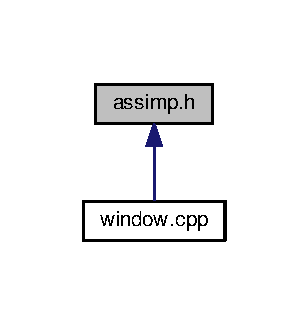
\includegraphics[width=148pt]{assimp_8h__dep__incl}
\end{center}
\end{figure}
\subsection*{Functions}
\begin{DoxyCompactItemize}
\item 
void \hyperlink{assimp_8h_aa57b10d56b7f497a1563c4c0d0a17889}{assimp\+Init} (const char $\ast$filename, unsigned int d)
\item 
void \hyperlink{assimp_8h_a981df57c9b37f7b881c9887edcba0a2b}{assimp\+Draw\+Scene} (unsigned int id)
\item 
void \hyperlink{assimp_8h_a0c1f6c204843bd061140485cb4387622}{assimp\+Quit} (void)
\end{DoxyCompactItemize}


\subsection{Detailed Description}
fonctionalit�s pour utilisation de lib Assimp sous G\+L4\+Dummies. 

\begin{DoxyAuthor}{Author}
Far�s B\+E\+L\+H\+A\+DJ, \href{mailto:amsi@ai.univ-paris8.fr}{\tt amsi@ai.\+univ-\/paris8.\+fr} 
\end{DoxyAuthor}
\begin{DoxyDate}{Date}
February 14, 2017 
\end{DoxyDate}


\subsection{Function Documentation}
\index{assimp.\+h@{assimp.\+h}!assimp\+Draw\+Scene@{assimp\+Draw\+Scene}}
\index{assimp\+Draw\+Scene@{assimp\+Draw\+Scene}!assimp.\+h@{assimp.\+h}}
\subsubsection[{\texorpdfstring{assimp\+Draw\+Scene(unsigned int id)}{assimpDrawScene(unsigned int id)}}]{\setlength{\rightskip}{0pt plus 5cm}void assimp\+Draw\+Scene (
\begin{DoxyParamCaption}
\item[{unsigned int}]{id}
\end{DoxyParamCaption}
)}\hypertarget{assimp_8h_a981df57c9b37f7b881c9887edcba0a2b}{}\label{assimp_8h_a981df57c9b37f7b881c9887edcba0a2b}
\index{assimp.\+h@{assimp.\+h}!assimp\+Init@{assimp\+Init}}
\index{assimp\+Init@{assimp\+Init}!assimp.\+h@{assimp.\+h}}
\subsubsection[{\texorpdfstring{assimp\+Init(const char $\ast$filename, unsigned int d)}{assimpInit(const char *filename, unsigned int d)}}]{\setlength{\rightskip}{0pt plus 5cm}void assimp\+Init (
\begin{DoxyParamCaption}
\item[{const char $\ast$}]{filename, }
\item[{unsigned int}]{d}
\end{DoxyParamCaption}
)}\hypertarget{assimp_8h_aa57b10d56b7f497a1563c4c0d0a17889}{}\label{assimp_8h_aa57b10d56b7f497a1563c4c0d0a17889}
\index{assimp.\+h@{assimp.\+h}!assimp\+Quit@{assimp\+Quit}}
\index{assimp\+Quit@{assimp\+Quit}!assimp.\+h@{assimp.\+h}}
\subsubsection[{\texorpdfstring{assimp\+Quit(void)}{assimpQuit(void)}}]{\setlength{\rightskip}{0pt plus 5cm}void assimp\+Quit (
\begin{DoxyParamCaption}
\item[{void}]{}
\end{DoxyParamCaption}
)}\hypertarget{assimp_8h_a0c1f6c204843bd061140485cb4387622}{}\label{assimp_8h_a0c1f6c204843bd061140485cb4387622}

\hypertarget{assimp__log_8txt}{}\section{assimp\+\_\+log.\+txt File Reference}
\label{assimp__log_8txt}\index{assimp\+\_\+log.\+txt@{assimp\+\_\+log.\+txt}}
\subsection*{Variables}
\begin{DoxyCompactItemize}
\item 
\hyperlink{assimp__log_8txt_a10e136332d6dc091c13986d59367f7a1}{Info}
\item 
\hyperlink{assimp__log_8txt_a4f6b0da32d987d712f99f108a27b44ff}{T0} \hyperlink{assimp__log_8txt_acdfe4734f16c9d3b3fc5affb4fefed6e}{\+\_\+\+\_\+pad0\+\_\+\+\_\+}
\item 
T0 \hyperlink{assimp__log_8txt_a4f6b0da32d987d712f99f108a27b44ff}{T0}
\item 
\hyperlink{assimp__log_8txt_a4f6b0da32d987d712f99f108a27b44ff}{T0} \hyperlink{assimp__log_8txt_a45fe61d4047cde49c4946edc0d1ac62e}{Lines}
\item 
\hyperlink{assimp__log_8txt_a4f6b0da32d987d712f99f108a27b44ff}{T0} \hyperlink{assimp__log_8txt_a11eaa1907dff68316087b51244ae7d9f}{Triangles}
\item 
\hyperlink{assimp__log_8txt_a4f6b0da32d987d712f99f108a27b44ff}{T0} \hyperlink{assimp__log_8txt_afa6022965f219ff3e1a1319e791de3a4}{Polygons}
\end{DoxyCompactItemize}


\subsection{Variable Documentation}
\index{assimp\+\_\+log.\+txt@{assimp\+\_\+log.\+txt}!\+\_\+\+\_\+pad0\+\_\+\+\_\+@{\+\_\+\+\_\+pad0\+\_\+\+\_\+}}
\index{\+\_\+\+\_\+pad0\+\_\+\+\_\+@{\+\_\+\+\_\+pad0\+\_\+\+\_\+}!assimp\+\_\+log.\+txt@{assimp\+\_\+log.\+txt}}
\subsubsection[{\texorpdfstring{\+\_\+\+\_\+pad0\+\_\+\+\_\+}{__pad0__}}]{\setlength{\rightskip}{0pt plus 5cm}{\bf T0} \+\_\+\+\_\+pad0\+\_\+\+\_\+}\hypertarget{assimp__log_8txt_acdfe4734f16c9d3b3fc5affb4fefed6e}{}\label{assimp__log_8txt_acdfe4734f16c9d3b3fc5affb4fefed6e}
\index{assimp\+\_\+log.\+txt@{assimp\+\_\+log.\+txt}!Info@{Info}}
\index{Info@{Info}!assimp\+\_\+log.\+txt@{assimp\+\_\+log.\+txt}}
\subsubsection[{\texorpdfstring{Info}{Info}}]{\setlength{\rightskip}{0pt plus 5cm}Info}\hypertarget{assimp__log_8txt_a10e136332d6dc091c13986d59367f7a1}{}\label{assimp__log_8txt_a10e136332d6dc091c13986d59367f7a1}
\index{assimp\+\_\+log.\+txt@{assimp\+\_\+log.\+txt}!Lines@{Lines}}
\index{Lines@{Lines}!assimp\+\_\+log.\+txt@{assimp\+\_\+log.\+txt}}
\subsubsection[{\texorpdfstring{Lines}{Lines}}]{\setlength{\rightskip}{0pt plus 5cm}{\bf T0} Lines}\hypertarget{assimp__log_8txt_a45fe61d4047cde49c4946edc0d1ac62e}{}\label{assimp__log_8txt_a45fe61d4047cde49c4946edc0d1ac62e}
\index{assimp\+\_\+log.\+txt@{assimp\+\_\+log.\+txt}!Polygons@{Polygons}}
\index{Polygons@{Polygons}!assimp\+\_\+log.\+txt@{assimp\+\_\+log.\+txt}}
\subsubsection[{\texorpdfstring{Polygons}{Polygons}}]{\setlength{\rightskip}{0pt plus 5cm}{\bf T0} Polygons}\hypertarget{assimp__log_8txt_afa6022965f219ff3e1a1319e791de3a4}{}\label{assimp__log_8txt_afa6022965f219ff3e1a1319e791de3a4}
\index{assimp\+\_\+log.\+txt@{assimp\+\_\+log.\+txt}!T0@{T0}}
\index{T0@{T0}!assimp\+\_\+log.\+txt@{assimp\+\_\+log.\+txt}}
\subsubsection[{\texorpdfstring{T0}{T0}}]{\setlength{\rightskip}{0pt plus 5cm}T0 T0}\hypertarget{assimp__log_8txt_a4f6b0da32d987d712f99f108a27b44ff}{}\label{assimp__log_8txt_a4f6b0da32d987d712f99f108a27b44ff}
\index{assimp\+\_\+log.\+txt@{assimp\+\_\+log.\+txt}!Triangles@{Triangles}}
\index{Triangles@{Triangles}!assimp\+\_\+log.\+txt@{assimp\+\_\+log.\+txt}}
\subsubsection[{\texorpdfstring{Triangles}{Triangles}}]{\setlength{\rightskip}{0pt plus 5cm}{\bf T0} Triangles}\hypertarget{assimp__log_8txt_a11eaa1907dff68316087b51244ae7d9f}{}\label{assimp__log_8txt_a11eaa1907dff68316087b51244ae7d9f}

\hypertarget{window_8cpp}{}\section{window.\+cpp File Reference}
\label{window_8cpp}\index{window.\+cpp@{window.\+cpp}}
{\ttfamily \#include $<$opencv2/core/core.\+hpp$>$}\\*
{\ttfamily \#include $<$opencv2/highgui/highgui.\+hpp$>$}\\*
{\ttfamily \#include $<$opencv2/imgproc/imgproc.\+hpp$>$}\\*
{\ttfamily \#include $<$opencv2/objdetect.\+hpp$>$}\\*
{\ttfamily \#include $<$opencv2/videoio/videoio\+\_\+c.\+h$>$}\\*
{\ttfamily \#include $<$opencv2/opencv.\+hpp$>$}\\*
{\ttfamily \#include $<$iostream$>$}\\*
{\ttfamily \#include $<$G\+L4\+D/gl4du.\+h$>$}\\*
{\ttfamily \#include $<$G\+L4\+D/gl4dg.\+h$>$}\\*
{\ttfamily \#include $<$G\+L4\+D/gl4duw\+\_\+\+S\+D\+L2.\+h$>$}\\*
{\ttfamily \#include $<$S\+D\+L2/\+S\+D\+L\+\_\+image.\+h$>$}\\*
{\ttfamily \#include \char`\"{}assimp.\+h\char`\"{}}\\*
Include dependency graph for window.\+cpp\+:
\nopagebreak
\begin{figure}[H]
\begin{center}
\leavevmode
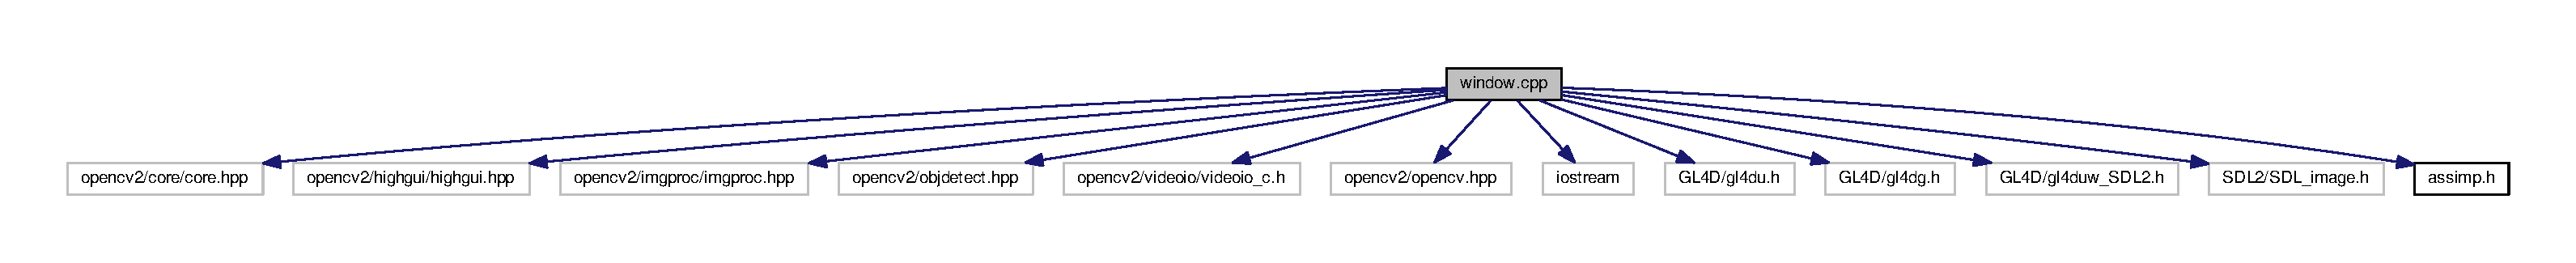
\includegraphics[width=350pt]{window_8cpp__incl}
\end{center}
\end{figure}
\subsection*{Functions}
\begin{DoxyCompactItemize}
\item 
static S\+D\+L\+\_\+\+Window $\ast$ \hyperlink{window_8cpp_a181784b514f1d71a5a7573068e7228be}{init\+Window} (int w, int h, S\+D\+L\+\_\+\+G\+L\+Context $\ast$pogl\+Context)
\item 
static void \hyperlink{window_8cpp_ac6d84025d3d3d48e5f7e418f877bd574}{init\+GL} (S\+D\+L\+\_\+\+Window $\ast$win)
\begin{DoxyCompactList}\small\item\em Cette fonction initialise les paramètres Open\+GL. \end{DoxyCompactList}\item 
static void \hyperlink{window_8cpp_ad6169536f88b2f942555ab20445c35bc}{init\+Data} (void)
\item 
static void \hyperlink{window_8cpp_a28d5ce82194141dd9dd4b874f6a8e0e9}{resize\+GL} (S\+D\+L\+\_\+\+Window $\ast$win)
\begin{DoxyCompactList}\small\item\em Cette fonction paramétrela vue (view\+Port) Open\+GL en fonction des dimensions de la fenêtre S\+DL pointée par {\itshape win}. \end{DoxyCompactList}\item 
static void \hyperlink{window_8cpp_a67a338c6f0e35065e524006b419fc1dd}{loop} (S\+D\+L\+\_\+\+Window $\ast$win)
\begin{DoxyCompactList}\small\item\em Boucle infinie principale \+: gère les évènements, dessine, imprime le F\+PS et swap les buffers. \end{DoxyCompactList}\item 
static void \hyperlink{window_8cpp_a96a68ee53ffcf494ca60f94ac05d94bb}{draw} (void)
\begin{DoxyCompactList}\small\item\em dessine dans le contexte Open\+GL actif. \end{DoxyCompactList}\item 
static void \hyperlink{window_8cpp_ae38367d7a4d4121f6d1693d61f7f905a}{quit} (void)
\begin{DoxyCompactList}\small\item\em appelée au moment de sortir du programme (atexit), libère les éléments utilisés \end{DoxyCompactList}\item 
static void \hyperlink{window_8cpp_a0c66ed924433ae3fd48567923eb68f8b}{translate\+\_\+coord} (G\+Lfloat $\ast$ip, int xm, int ym)
\begin{DoxyCompactList}\small\item\em traduit les coordonnees renvoyées par vector$<$\+Rect$>$, en coordonnees exploitables par le contexte Open\+GL. \end{DoxyCompactList}\item 
void \hyperlink{window_8cpp_a078cb023299d74a3abc79d470c261d7f}{assimp\+Objet} (G\+Lfloat x, G\+Lfloat y, G\+Lfloat z, G\+Lfloat theta, G\+Luint id)
\begin{DoxyCompactList}\small\item\em fonction qui dessine un object assimp \end{DoxyCompactList}\item 
int \hyperlink{window_8cpp_a3c04138a5bfe5d72780bb7e82a18e627}{main} (int argc, char $\ast$$\ast$argv)
\end{DoxyCompactItemize}
\subsection*{Variables}
\begin{DoxyCompactItemize}
\item 
static Cascade\+Classifier $\ast$ \hyperlink{window_8cpp_aef4b6d90b88c97e5c0ebf6c910513e6f}{face\+\_\+cc}
\item 
static Cascade\+Classifier $\ast$ \hyperlink{window_8cpp_a63dae8d0c40b453b371706b9e5e1b308}{eye\+\_\+cc}
\item 
static Cascade\+Classifier $\ast$ \hyperlink{window_8cpp_a03598e8e75d3a25756e1411bf559beb4}{nose\+\_\+cc}
\item 
static Mat \hyperlink{window_8cpp_a5edc9131429837d9b41dadc7a1cc7ee1}{camera\+Frame}
\item 
static int \hyperlink{window_8cpp_ac3fccedccc56d04d622b5745485a7568}{\+\_\+window\+Width} = 800
\begin{DoxyCompactList}\small\item\em dimensions de la fenêtre \end{DoxyCompactList}\item 
static int \hyperlink{window_8cpp_a5b25a069d46e2c8963f7a855f6a3582c}{\+\_\+window\+Height} = 600
\item 
static S\+D\+L\+\_\+\+Window $\ast$ \hyperlink{window_8cpp_a7178561b494fec72d25dda65624cbaad}{\+\_\+win} = N\+U\+LL
\begin{DoxyCompactList}\small\item\em pointeur vers la (future) fenêtre S\+DL \end{DoxyCompactList}\item 
static S\+D\+L\+\_\+\+G\+L\+Context \hyperlink{window_8cpp_a6663227b3085cc2fc62d845252017d7a}{\+\_\+ogl\+Context} = N\+U\+LL
\begin{DoxyCompactList}\small\item\em pointeur vers le (futur) contexte Open\+GL \end{DoxyCompactList}\item 
static G\+Luint \hyperlink{window_8cpp_ac1f4a1f92760da28a17a070c2a1aca23}{\+\_\+vao} = 0
\begin{DoxyCompactList}\small\item\em identifiant du (futur) vertex array object \end{DoxyCompactList}\item 
static G\+Luint \hyperlink{window_8cpp_a7437445160e76b84bd1e01368ec976da}{\+\_\+buffer} = 0
\begin{DoxyCompactList}\small\item\em identifiant du (futur) buffer de data \end{DoxyCompactList}\item 
static G\+Luint \hyperlink{window_8cpp_ac7ef75a87c3fccc7a1350bfc7167b5d5}{\+\_\+p\+Id} = 0
\begin{DoxyCompactList}\small\item\em identifiants des (futurs) G\+L\+SL programs \end{DoxyCompactList}\item 
static G\+Luint \hyperlink{window_8cpp_ac5b39e53d543f4ff963671f66d726665}{\+\_\+obj\+\_\+p\+Id} = 0
\item 
static G\+Luint \hyperlink{window_8cpp_ab084f8bfaed48bc9a6886602353d42e2}{\+\_\+t\+Id} = 0
\begin{DoxyCompactList}\small\item\em identifiant de la texture chargée \end{DoxyCompactList}\item 
static Video\+Capture $\ast$ \hyperlink{window_8cpp_a6dac95f98f7d2e9b479c55da65fa5120}{camera} = N\+U\+LL
\begin{DoxyCompactList}\small\item\em device de capture vidéo \end{DoxyCompactList}\end{DoxyCompactItemize}


\subsection{Function Documentation}
\index{window.\+cpp@{window.\+cpp}!assimp\+Objet@{assimp\+Objet}}
\index{assimp\+Objet@{assimp\+Objet}!window.\+cpp@{window.\+cpp}}
\subsubsection[{\texorpdfstring{assimp\+Objet(\+G\+Lfloat x, G\+Lfloat y, G\+Lfloat z, G\+Lfloat theta, G\+Luint id)}{assimpObjet(GLfloat x, GLfloat y, GLfloat z, GLfloat theta, GLuint id)}}]{\setlength{\rightskip}{0pt plus 5cm}void assimp\+Objet (
\begin{DoxyParamCaption}
\item[{G\+Lfloat}]{x, }
\item[{G\+Lfloat}]{y, }
\item[{G\+Lfloat}]{z, }
\item[{G\+Lfloat}]{theta, }
\item[{G\+Luint}]{id}
\end{DoxyParamCaption}
)}\hypertarget{window_8cpp_a078cb023299d74a3abc79d470c261d7f}{}\label{window_8cpp_a078cb023299d74a3abc79d470c261d7f}


fonction qui dessine un object assimp 


\begin{DoxyParams}{Parameters}
{\em x,y,z,theta} & et l\textquotesingle{}id de notre object \\
\hline
\end{DoxyParams}
\index{window.\+cpp@{window.\+cpp}!draw@{draw}}
\index{draw@{draw}!window.\+cpp@{window.\+cpp}}
\subsubsection[{\texorpdfstring{draw(void)}{draw(void)}}]{\setlength{\rightskip}{0pt plus 5cm}static void draw (
\begin{DoxyParamCaption}
\item[{void}]{}
\end{DoxyParamCaption}
)\hspace{0.3cm}{\ttfamily [static]}}\hypertarget{window_8cpp_a96a68ee53ffcf494ca60f94ac05d94bb}{}\label{window_8cpp_a96a68ee53ffcf494ca60f94ac05d94bb}


dessine dans le contexte Open\+GL actif. 

\index{window.\+cpp@{window.\+cpp}!init\+Data@{init\+Data}}
\index{init\+Data@{init\+Data}!window.\+cpp@{window.\+cpp}}
\subsubsection[{\texorpdfstring{init\+Data(void)}{initData(void)}}]{\setlength{\rightskip}{0pt plus 5cm}static void init\+Data (
\begin{DoxyParamCaption}
\item[{void}]{}
\end{DoxyParamCaption}
)\hspace{0.3cm}{\ttfamily [static]}}\hypertarget{window_8cpp_ad6169536f88b2f942555ab20445c35bc}{}\label{window_8cpp_ad6169536f88b2f942555ab20445c35bc}
\index{window.\+cpp@{window.\+cpp}!init\+GL@{init\+GL}}
\index{init\+GL@{init\+GL}!window.\+cpp@{window.\+cpp}}
\subsubsection[{\texorpdfstring{init\+G\+L(\+S\+D\+L\+\_\+\+Window $\ast$win)}{initGL(SDL_Window *win)}}]{\setlength{\rightskip}{0pt plus 5cm}static void init\+GL (
\begin{DoxyParamCaption}
\item[{S\+D\+L\+\_\+\+Window $\ast$}]{win}
\end{DoxyParamCaption}
)\hspace{0.3cm}{\ttfamily [static]}}\hypertarget{window_8cpp_ac6d84025d3d3d48e5f7e418f877bd574}{}\label{window_8cpp_ac6d84025d3d3d48e5f7e418f877bd574}


Cette fonction initialise les paramètres Open\+GL. 


\begin{DoxyParams}{Parameters}
{\em win} & le pointeur vers la fenêtre S\+DL pour laquelle nous avons attaché le contexte Open\+GL. \\
\hline
\end{DoxyParams}
\index{window.\+cpp@{window.\+cpp}!init\+Window@{init\+Window}}
\index{init\+Window@{init\+Window}!window.\+cpp@{window.\+cpp}}
\subsubsection[{\texorpdfstring{init\+Window(int w, int h, S\+D\+L\+\_\+\+G\+L\+Context $\ast$pogl\+Context)}{initWindow(int w, int h, SDL_GLContext *poglContext)}}]{\setlength{\rightskip}{0pt plus 5cm}static S\+D\+L\+\_\+\+Window $\ast$ init\+Window (
\begin{DoxyParamCaption}
\item[{int}]{w, }
\item[{int}]{h, }
\item[{S\+D\+L\+\_\+\+G\+L\+Context $\ast$}]{pogl\+Context}
\end{DoxyParamCaption}
)\hspace{0.3cm}{\ttfamily [static]}}\hypertarget{window_8cpp_a181784b514f1d71a5a7573068e7228be}{}\label{window_8cpp_a181784b514f1d71a5a7573068e7228be}
\index{window.\+cpp@{window.\+cpp}!loop@{loop}}
\index{loop@{loop}!window.\+cpp@{window.\+cpp}}
\subsubsection[{\texorpdfstring{loop(\+S\+D\+L\+\_\+\+Window $\ast$win)}{loop(SDL_Window *win)}}]{\setlength{\rightskip}{0pt plus 5cm}static void loop (
\begin{DoxyParamCaption}
\item[{S\+D\+L\+\_\+\+Window $\ast$}]{win}
\end{DoxyParamCaption}
)\hspace{0.3cm}{\ttfamily [static]}}\hypertarget{window_8cpp_a67a338c6f0e35065e524006b419fc1dd}{}\label{window_8cpp_a67a338c6f0e35065e524006b419fc1dd}


Boucle infinie principale \+: gère les évènements, dessine, imprime le F\+PS et swap les buffers. 


\begin{DoxyParams}{Parameters}
{\em win} & le pointeur vers la fenêtre S\+DL pour laquelle nous avons attaché le contexte Open\+GL. \\
\hline
\end{DoxyParams}
\index{window.\+cpp@{window.\+cpp}!main@{main}}
\index{main@{main}!window.\+cpp@{window.\+cpp}}
\subsubsection[{\texorpdfstring{main(int argc, char $\ast$$\ast$argv)}{main(int argc, char **argv)}}]{\setlength{\rightskip}{0pt plus 5cm}int main (
\begin{DoxyParamCaption}
\item[{int}]{argc, }
\item[{char $\ast$$\ast$}]{argv}
\end{DoxyParamCaption}
)}\hypertarget{window_8cpp_a3c04138a5bfe5d72780bb7e82a18e627}{}\label{window_8cpp_a3c04138a5bfe5d72780bb7e82a18e627}
\index{window.\+cpp@{window.\+cpp}!quit@{quit}}
\index{quit@{quit}!window.\+cpp@{window.\+cpp}}
\subsubsection[{\texorpdfstring{quit(void)}{quit(void)}}]{\setlength{\rightskip}{0pt plus 5cm}static void quit (
\begin{DoxyParamCaption}
\item[{void}]{}
\end{DoxyParamCaption}
)\hspace{0.3cm}{\ttfamily [static]}}\hypertarget{window_8cpp_ae38367d7a4d4121f6d1693d61f7f905a}{}\label{window_8cpp_ae38367d7a4d4121f6d1693d61f7f905a}


appelée au moment de sortir du programme (atexit), libère les éléments utilisés 

\index{window.\+cpp@{window.\+cpp}!resize\+GL@{resize\+GL}}
\index{resize\+GL@{resize\+GL}!window.\+cpp@{window.\+cpp}}
\subsubsection[{\texorpdfstring{resize\+G\+L(\+S\+D\+L\+\_\+\+Window $\ast$win)}{resizeGL(SDL_Window *win)}}]{\setlength{\rightskip}{0pt plus 5cm}static void resize\+GL (
\begin{DoxyParamCaption}
\item[{S\+D\+L\+\_\+\+Window $\ast$}]{win}
\end{DoxyParamCaption}
)\hspace{0.3cm}{\ttfamily [static]}}\hypertarget{window_8cpp_a28d5ce82194141dd9dd4b874f6a8e0e9}{}\label{window_8cpp_a28d5ce82194141dd9dd4b874f6a8e0e9}


Cette fonction paramétrela vue (view\+Port) Open\+GL en fonction des dimensions de la fenêtre S\+DL pointée par {\itshape win}. 


\begin{DoxyParams}{Parameters}
{\em win} & le pointeur vers la fenêtre S\+DL pour laquelle nous avons attaché le contexte Open\+GL. \\
\hline
\end{DoxyParams}
\index{window.\+cpp@{window.\+cpp}!translate\+\_\+coord@{translate\+\_\+coord}}
\index{translate\+\_\+coord@{translate\+\_\+coord}!window.\+cpp@{window.\+cpp}}
\subsubsection[{\texorpdfstring{translate\+\_\+coord(\+G\+Lfloat $\ast$ip, int xm, int ym)}{translate_coord(GLfloat *ip, int xm, int ym)}}]{\setlength{\rightskip}{0pt plus 5cm}static void translate\+\_\+coord (
\begin{DoxyParamCaption}
\item[{G\+Lfloat $\ast$}]{ip, }
\item[{int}]{xm, }
\item[{int}]{ym}
\end{DoxyParamCaption}
)\hspace{0.3cm}{\ttfamily [static]}}\hypertarget{window_8cpp_a0c66ed924433ae3fd48567923eb68f8b}{}\label{window_8cpp_a0c66ed924433ae3fd48567923eb68f8b}


traduit les coordonnees renvoyées par vector$<$\+Rect$>$, en coordonnees exploitables par le contexte Open\+GL. 


\begin{DoxyParams}{Parameters}
{\em pointeur} & ip\+: tableau contenant le x,y et z que l\textquotesingle{}on rempli dans la fonction valeur x de Rect valeur y de Rect \\
\hline
\end{DoxyParams}


\subsection{Variable Documentation}
\index{window.\+cpp@{window.\+cpp}!\+\_\+buffer@{\+\_\+buffer}}
\index{\+\_\+buffer@{\+\_\+buffer}!window.\+cpp@{window.\+cpp}}
\subsubsection[{\texorpdfstring{\+\_\+buffer}{_buffer}}]{\setlength{\rightskip}{0pt plus 5cm}G\+Luint \+\_\+buffer = 0\hspace{0.3cm}{\ttfamily [static]}}\hypertarget{window_8cpp_a7437445160e76b84bd1e01368ec976da}{}\label{window_8cpp_a7437445160e76b84bd1e01368ec976da}


identifiant du (futur) buffer de data 

\index{window.\+cpp@{window.\+cpp}!\+\_\+obj\+\_\+p\+Id@{\+\_\+obj\+\_\+p\+Id}}
\index{\+\_\+obj\+\_\+p\+Id@{\+\_\+obj\+\_\+p\+Id}!window.\+cpp@{window.\+cpp}}
\subsubsection[{\texorpdfstring{\+\_\+obj\+\_\+p\+Id}{_obj_pId}}]{\setlength{\rightskip}{0pt plus 5cm}G\+Luint \+\_\+obj\+\_\+p\+Id = 0\hspace{0.3cm}{\ttfamily [static]}}\hypertarget{window_8cpp_ac5b39e53d543f4ff963671f66d726665}{}\label{window_8cpp_ac5b39e53d543f4ff963671f66d726665}
\index{window.\+cpp@{window.\+cpp}!\+\_\+ogl\+Context@{\+\_\+ogl\+Context}}
\index{\+\_\+ogl\+Context@{\+\_\+ogl\+Context}!window.\+cpp@{window.\+cpp}}
\subsubsection[{\texorpdfstring{\+\_\+ogl\+Context}{_oglContext}}]{\setlength{\rightskip}{0pt plus 5cm}S\+D\+L\+\_\+\+G\+L\+Context \+\_\+ogl\+Context = N\+U\+LL\hspace{0.3cm}{\ttfamily [static]}}\hypertarget{window_8cpp_a6663227b3085cc2fc62d845252017d7a}{}\label{window_8cpp_a6663227b3085cc2fc62d845252017d7a}


pointeur vers le (futur) contexte Open\+GL 

\index{window.\+cpp@{window.\+cpp}!\+\_\+p\+Id@{\+\_\+p\+Id}}
\index{\+\_\+p\+Id@{\+\_\+p\+Id}!window.\+cpp@{window.\+cpp}}
\subsubsection[{\texorpdfstring{\+\_\+p\+Id}{_pId}}]{\setlength{\rightskip}{0pt plus 5cm}G\+Luint \+\_\+p\+Id = 0\hspace{0.3cm}{\ttfamily [static]}}\hypertarget{window_8cpp_ac7ef75a87c3fccc7a1350bfc7167b5d5}{}\label{window_8cpp_ac7ef75a87c3fccc7a1350bfc7167b5d5}


identifiants des (futurs) G\+L\+SL programs 

\index{window.\+cpp@{window.\+cpp}!\+\_\+t\+Id@{\+\_\+t\+Id}}
\index{\+\_\+t\+Id@{\+\_\+t\+Id}!window.\+cpp@{window.\+cpp}}
\subsubsection[{\texorpdfstring{\+\_\+t\+Id}{_tId}}]{\setlength{\rightskip}{0pt plus 5cm}G\+Luint \+\_\+t\+Id = 0\hspace{0.3cm}{\ttfamily [static]}}\hypertarget{window_8cpp_ab084f8bfaed48bc9a6886602353d42e2}{}\label{window_8cpp_ab084f8bfaed48bc9a6886602353d42e2}


identifiant de la texture chargée 

\index{window.\+cpp@{window.\+cpp}!\+\_\+vao@{\+\_\+vao}}
\index{\+\_\+vao@{\+\_\+vao}!window.\+cpp@{window.\+cpp}}
\subsubsection[{\texorpdfstring{\+\_\+vao}{_vao}}]{\setlength{\rightskip}{0pt plus 5cm}G\+Luint \+\_\+vao = 0\hspace{0.3cm}{\ttfamily [static]}}\hypertarget{window_8cpp_ac1f4a1f92760da28a17a070c2a1aca23}{}\label{window_8cpp_ac1f4a1f92760da28a17a070c2a1aca23}


identifiant du (futur) vertex array object 

\index{window.\+cpp@{window.\+cpp}!\+\_\+win@{\+\_\+win}}
\index{\+\_\+win@{\+\_\+win}!window.\+cpp@{window.\+cpp}}
\subsubsection[{\texorpdfstring{\+\_\+win}{_win}}]{\setlength{\rightskip}{0pt plus 5cm}S\+D\+L\+\_\+\+Window$\ast$ \+\_\+win = N\+U\+LL\hspace{0.3cm}{\ttfamily [static]}}\hypertarget{window_8cpp_a7178561b494fec72d25dda65624cbaad}{}\label{window_8cpp_a7178561b494fec72d25dda65624cbaad}


pointeur vers la (future) fenêtre S\+DL 

\index{window.\+cpp@{window.\+cpp}!\+\_\+window\+Height@{\+\_\+window\+Height}}
\index{\+\_\+window\+Height@{\+\_\+window\+Height}!window.\+cpp@{window.\+cpp}}
\subsubsection[{\texorpdfstring{\+\_\+window\+Height}{_windowHeight}}]{\setlength{\rightskip}{0pt plus 5cm}int \+\_\+window\+Height = 600\hspace{0.3cm}{\ttfamily [static]}}\hypertarget{window_8cpp_a5b25a069d46e2c8963f7a855f6a3582c}{}\label{window_8cpp_a5b25a069d46e2c8963f7a855f6a3582c}
\index{window.\+cpp@{window.\+cpp}!\+\_\+window\+Width@{\+\_\+window\+Width}}
\index{\+\_\+window\+Width@{\+\_\+window\+Width}!window.\+cpp@{window.\+cpp}}
\subsubsection[{\texorpdfstring{\+\_\+window\+Width}{_windowWidth}}]{\setlength{\rightskip}{0pt plus 5cm}int \+\_\+window\+Width = 800\hspace{0.3cm}{\ttfamily [static]}}\hypertarget{window_8cpp_ac3fccedccc56d04d622b5745485a7568}{}\label{window_8cpp_ac3fccedccc56d04d622b5745485a7568}


dimensions de la fenêtre 

\index{window.\+cpp@{window.\+cpp}!camera@{camera}}
\index{camera@{camera}!window.\+cpp@{window.\+cpp}}
\subsubsection[{\texorpdfstring{camera}{camera}}]{\setlength{\rightskip}{0pt plus 5cm}Video\+Capture$\ast$ camera = N\+U\+LL\hspace{0.3cm}{\ttfamily [static]}}\hypertarget{window_8cpp_a6dac95f98f7d2e9b479c55da65fa5120}{}\label{window_8cpp_a6dac95f98f7d2e9b479c55da65fa5120}


device de capture vidéo 

\index{window.\+cpp@{window.\+cpp}!camera\+Frame@{camera\+Frame}}
\index{camera\+Frame@{camera\+Frame}!window.\+cpp@{window.\+cpp}}
\subsubsection[{\texorpdfstring{camera\+Frame}{cameraFrame}}]{\setlength{\rightskip}{0pt plus 5cm}Mat camera\+Frame\hspace{0.3cm}{\ttfamily [static]}}\hypertarget{window_8cpp_a5edc9131429837d9b41dadc7a1cc7ee1}{}\label{window_8cpp_a5edc9131429837d9b41dadc7a1cc7ee1}
\index{window.\+cpp@{window.\+cpp}!eye\+\_\+cc@{eye\+\_\+cc}}
\index{eye\+\_\+cc@{eye\+\_\+cc}!window.\+cpp@{window.\+cpp}}
\subsubsection[{\texorpdfstring{eye\+\_\+cc}{eye_cc}}]{\setlength{\rightskip}{0pt plus 5cm}Cascade\+Classifier$\ast$ eye\+\_\+cc\hspace{0.3cm}{\ttfamily [static]}}\hypertarget{window_8cpp_a63dae8d0c40b453b371706b9e5e1b308}{}\label{window_8cpp_a63dae8d0c40b453b371706b9e5e1b308}
\index{window.\+cpp@{window.\+cpp}!face\+\_\+cc@{face\+\_\+cc}}
\index{face\+\_\+cc@{face\+\_\+cc}!window.\+cpp@{window.\+cpp}}
\subsubsection[{\texorpdfstring{face\+\_\+cc}{face_cc}}]{\setlength{\rightskip}{0pt plus 5cm}Cascade\+Classifier$\ast$ face\+\_\+cc\hspace{0.3cm}{\ttfamily [static]}}\hypertarget{window_8cpp_aef4b6d90b88c97e5c0ebf6c910513e6f}{}\label{window_8cpp_aef4b6d90b88c97e5c0ebf6c910513e6f}
\index{window.\+cpp@{window.\+cpp}!nose\+\_\+cc@{nose\+\_\+cc}}
\index{nose\+\_\+cc@{nose\+\_\+cc}!window.\+cpp@{window.\+cpp}}
\subsubsection[{\texorpdfstring{nose\+\_\+cc}{nose_cc}}]{\setlength{\rightskip}{0pt plus 5cm}Cascade\+Classifier$\ast$ nose\+\_\+cc\hspace{0.3cm}{\ttfamily [static]}}\hypertarget{window_8cpp_a03598e8e75d3a25756e1411bf559beb4}{}\label{window_8cpp_a03598e8e75d3a25756e1411bf559beb4}

%--- End generated contents ---

% Index
\backmatter
\newpage
\phantomsection
\clearemptydoublepage
\addcontentsline{toc}{chapter}{Index}
\printindex

\end{document}
